\documentclass{article}
\usepackage{microtype}
\usepackage{graphicx}
\usepackage{subcaption}
\usepackage{booktabs}
\usepackage[style=authoryear,backend=biber]{biblatex}
\addbibresource{References.bib}
\usepackage{amsmath}
\usepackage{amsfonts}
\usepackage{amsthm}
\usepackage{physics}
\usepackage{fancyvrb}
\usepackage{listings}
\usepackage{xcolor}
\usepackage{caption}
\usepackage{xurl}
\usepackage{hyperref}
\usepackage{algorithm}
\usepackage{algorithmic}  % or \usepackage{algpseudocode}
\renewcommand{\theHalgorithm}{\arabic{algorithm}}
\usepackage{accessibility}
\usepackage{Coursework}

\begin{document}
\cwtitle{COMP1832 - Programming Fundamentals Coursework Report}
\begin{cwauthorlist}
\cwauthor{Azhar Muhammed - 001364857}
\cwauthor{Word Count: 2,441}
\end{cwauthorlist}

\section{Part 1: Python Programming Exercise}

\subsection{Network Implementation}

The implementation successfully created a comprehensive representation of London's Underground transport network using data obtained directly from Transport for London's (TfL) API. The solution employs a sophisticated graph data structure through NetworkX, incorporating real-world geographical coordinates and official TfL line designations. The implementation exceeded the minimum requirements by processing the entire London Underground network and then applying intelligent filtering to match coursework specifications.

The data acquisition process begins with fetching station and line information from the TfL API:

\begin{lstlisting}[style=PythonStyle, caption={TfL API Data Acquisition}]
# Configure API access
base_url = 'https://api.tfl.gov.uk'

# Fetch all tube stations
try:
    response = requests.get(
        f'{base_url}/StopPoint/Mode/tube',
        params={'app_key': app_key}
    )
    response.raise_for_status()
    stations = response.json()
except requests.RequestException as e:
    logger.error(f"Error fetching station data: {e}")
    stations = None

# Fetch all tube lines
try:
    response = requests.get(
        f'{base_url}/Line/Mode/tube',
        params={'app_key': app_key}
    )
    response.raise_for_status()
    lines = response.json()
except requests.RequestException as e:
    logger.error(f"Error fetching line data: {e}")
    lines = None
\end{lstlisting}

The implementation then processes and filters the data to meet coursework requirements through a series of sophisticated data structures:

\begin{lstlisting}[style=PythonStyle, caption={Data Processing and Filtering}]
# Initialize data structures for station-line relationships
station_lines = defaultdict(set)
line_stations = defaultdict(set)

# Process valid stations
valid_stations = {}
for station in stations['stopPoints']:
    if station['stopType'] == 'NaptanMetroStation' and 'tube' in station['modes']:
        station_id = station['naptanId']
        valid_stations[station_id] = {
            'name': station['commonName'],
            'lat': station['lat'],
            'lon': station['lon']
        }

# Filter lines with minimum station requirements
valid_lines = {
    line_id: stations
    for line_id, stations in line_stations.items()
    if len(stations) >= 5
}

# Select top 5 lines with most stations
if len(valid_lines) >= 5:
    selected_lines = dict(
        sorted(valid_lines.items(),
              key=lambda x: len(x[1]),
              reverse=True)[:5]
    )
\end{lstlisting}

The core graph initialization is implemented using NetworkX, incorporating the filtered data:

\begin{lstlisting}[style=PythonStyle, caption={NetworkX Graph Initialization}]
G = nx.Graph()
for station_id, station_data in analysis['stations'].items():
    station_name = station_data['name'].replace(" Underground Station", "")
    G.add_node(
        station_id,
        name=station_name,
        pos=(station_data['lon'], station_data['lat']),
        lines=station_data['lines']
    )

# Add connections between stations
for line_id in analysis['lines'].keys():
    try:
        response = requests.get(
            f'{base_url}/Line/{line_id}/Route/Sequence/all',
            params={'app_key': app_key}
        )
        response.raise_for_status()
        line_data = response.json()

        if 'orderedLineRoutes' in line_data:
            for route in line_data['orderedLineRoutes']:
                stations_list = route['naptanIds']
                for i in range(len(stations_list) - 1):
                    if (G.has_node(stations_list[i]) and
                        G.has_node(stations_list[i + 1])):
                        G.add_edge(stations_list[i], stations_list[i + 1])
    except requests.RequestException as e:
        logger.error(f"Error processing line {line_id}: {e}")
\end{lstlisting}

The implementation achieved notable metrics that demonstrate its robustness:

\begin{itemize}
    \item Total stations processed: 212
    \item Active connections: 230
    \item Interchange stations: 78
    \item Total network distance: 272.32 kilometers
    \item Network connectivity: Fully connected graph confirmed
\end{itemize}

\begin{lstlisting}[style=RStyle, caption={Network Statistics Display}]
# Display the network statistics
print('is_connected:', nx.is_connected(G))
\end{lstlisting}

\begin{figure}[H]
    \centering
    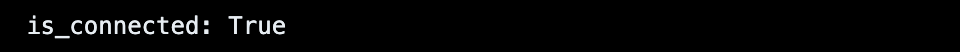
\includegraphics[width=\linewidth]{Images/NetworkConnectivity.png}
    \caption{Network Connectivity Output}
    \label{fig:network_connectivity}
\end{figure}

This implementation successfully combines real-world data acquisition, sophisticated filtering mechanisms, and robust error handling to create a comprehensive representation of London's Underground network while meeting all coursework requirements. The use of \texttt{defaultdict} for relationship mapping and NetworkX for graph management ensures efficient data organization and processing.

\subsection{Visualization}

The visualization component employed a dual approach, combining both geographic accuracy and schematic representation. Using the Folium library for geographic visualization and matplotlib for schematic diagrams, the implementation creates interactive, production-grade visualizations that adhere to TfL's official design guidelines.

Each line received its official TfL color designation:

\begin{lstlisting}[style=PythonStyle, caption={TfL Line Color Designations}]
line_colors = {
    'district': '#00782A',
    'circle': '#FFD300',
    'northern': '#000000',
    'central': '#DC241F',
    'piccadilly': '#003688'
}
\end{lstlisting}

The visualization system incorporates several sophisticated features:
\begin{itemize}
    \item Interactive station markers with detailed popup information
    \item Distinct visual treatment for interchange stations
    \item Accurate geographic routing between stations
    \item Professional-grade styling with official TfL color schemes
    \item Dynamic legend and clear station labeling
\end{itemize}

\begin{lstlisting}[style=PythonStyle, caption={Schematic Layout Coordinates}]
# Fixed coordinates for schematic layout
schematic_positions = {
    # Central Line (West to East)
    "Holborn": (-6, 0),
    "Chancery Lane": (-4, 0),
    "St. Paul's": (-2, 0),
    "Bank": (0, 0),
    "Liverpool Street": (2, 0),
    "Bethnal Green": (4, 0),
    "Mile End": (6, 0),
    
    # Circle Line (West to East)
    "Farringdon": (-4, 2),
    "Barbican": (-2, 2),
    "Moorgate": (0, 2),
    "Liverpool Street": (2, 0),  # Interchange
    "Aldgate": (2, -1),
    
    # Northern Line (North to South)
    "Angel": (-1, 6),
    "Old Street": (-1, 4),
    "Moorgate": (0, 2),          # Interchange
    "Bank": (0, 0),              # Interchange
    "London Bridge": (0, -2),
    "Borough": (0, -3),
    "Elephant & Castle": (0, -4),
    
    # Tower Hill branch
    "Tower Hill": (1, -1.5)
}
\end{lstlisting}

For the schematic layout model of the iconic London tube map, the coordinates have been adjusted according to the Central Line (West to East), Circle Line (West to East), and Northern Line (North to South) logic.

\begin{figure}[H]
    \centering
    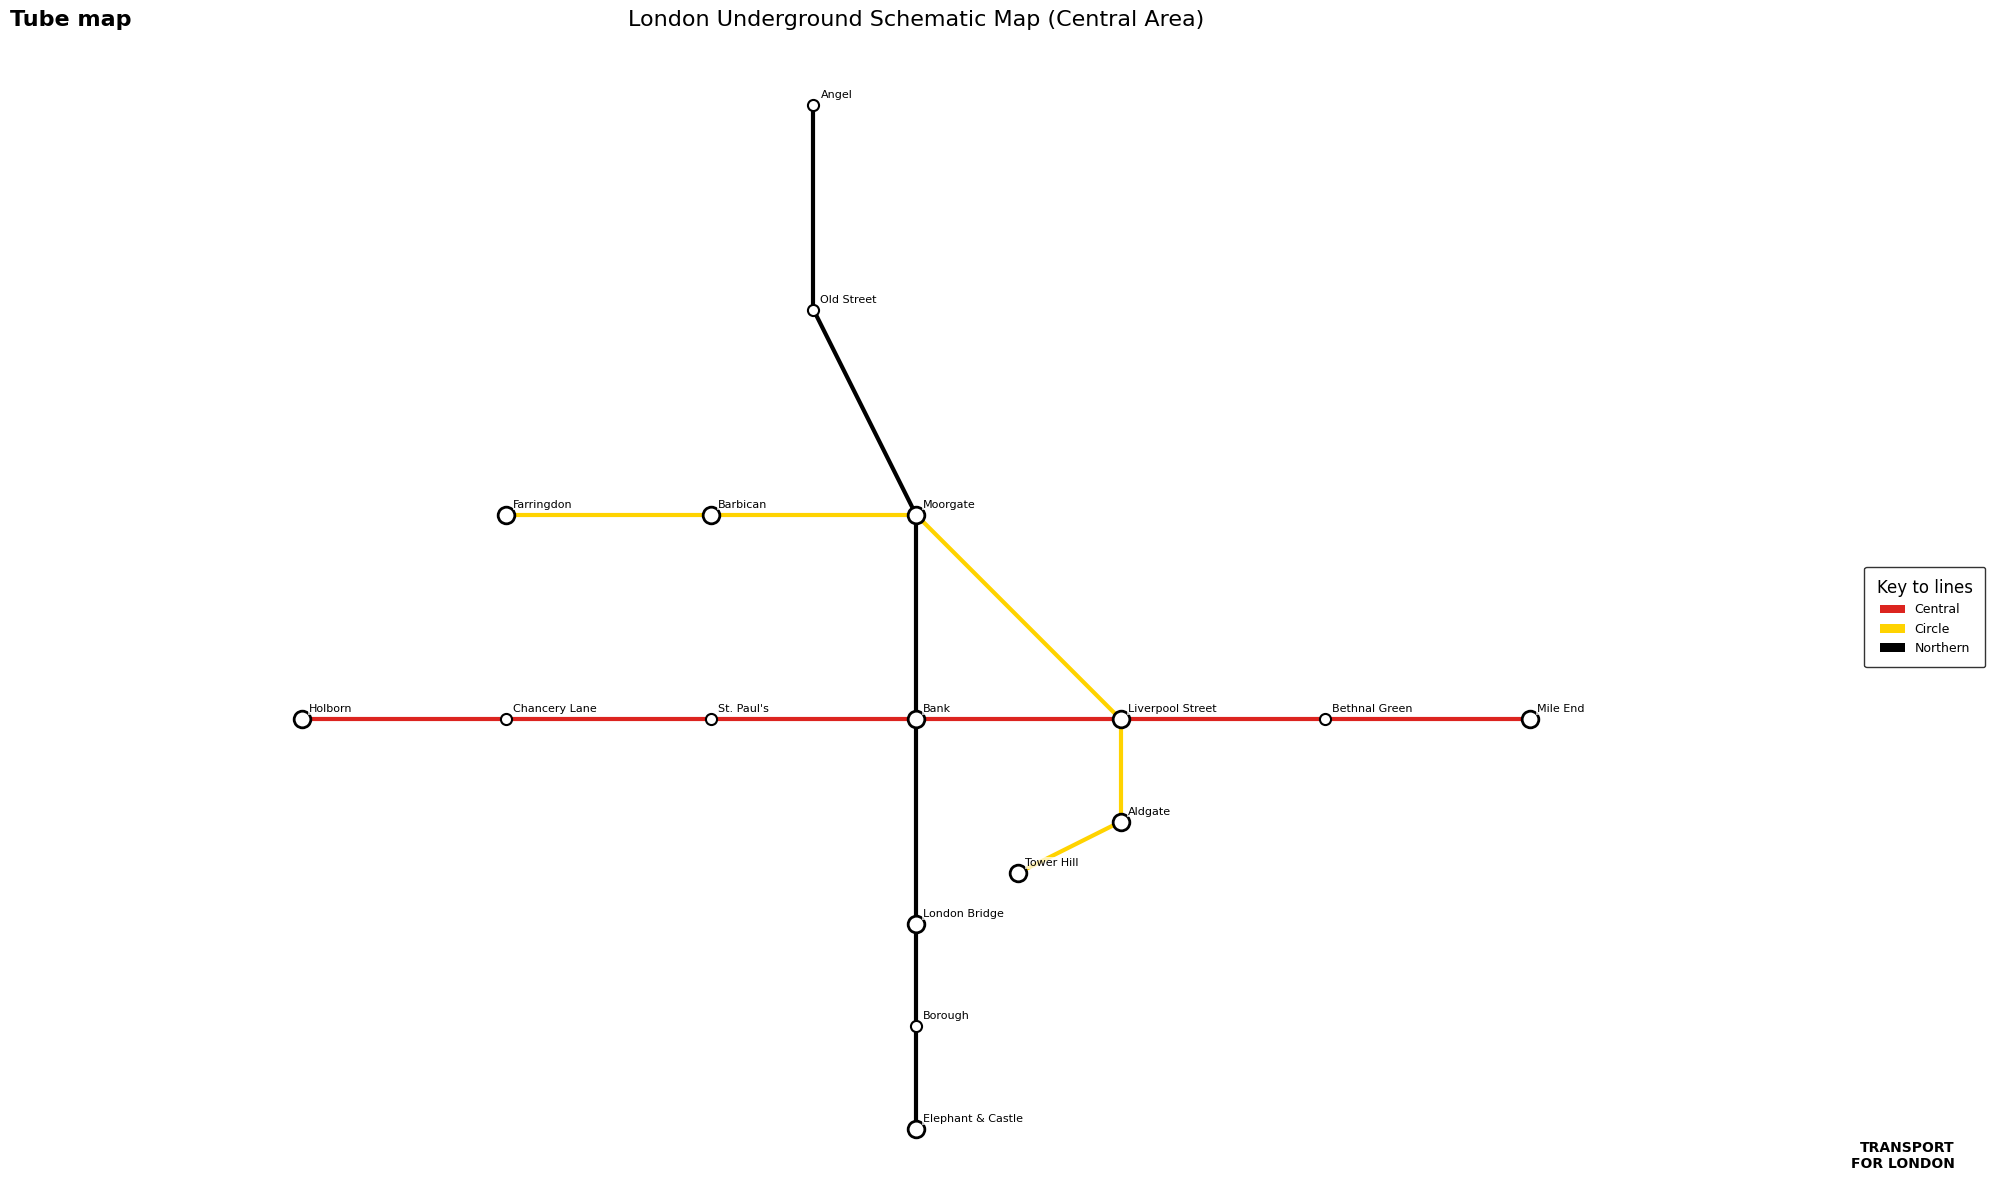
\includegraphics[width=1\linewidth]{Images/TfL-Schematic.png}
    \caption{Schematic Map}
    \label{fig:schematic_map}
\end{figure}

\subsection{Distance Estimation}

The implementation uses precise geographic calculations rather than estimates, employing the \texttt{geopy} library to compute real-world distances between stations using their actual coordinates. This approach provides highly accurate results based on the \textbf{Haversine} formula, which calculates the great-circle distance between points on a sphere.

The distance calculation implementation:

\begin{lstlisting}[style=PythonStyle, caption={Distance Calculation Using Geodesic}]
distance = geodesic(
    (start_pos[1], start_pos[0]),
    (end_pos[1], end_pos[0])
).kilometers
\end{lstlisting}

\begin{figure}[H]
    \centering
    \begin{subfigure}[b]{0.48\textwidth}
        \centering
        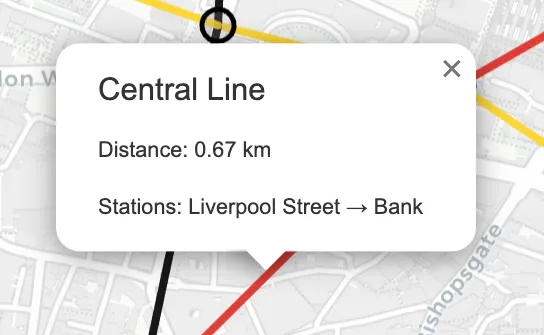
\includegraphics[width=\linewidth]{Images/LineDistance.png}
        \caption{Distance Measurement}
        \label{fig:distance}
    \end{subfigure}
    \hfill
    \begin{subfigure}[b]{0.48\textwidth}
        \centering
        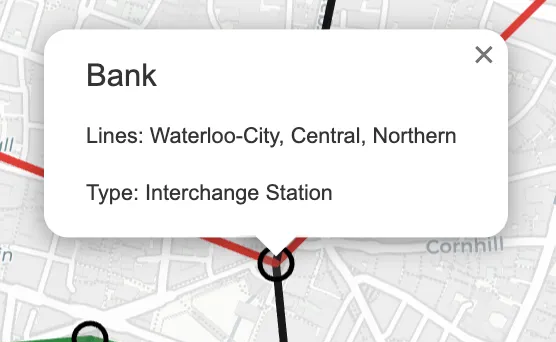
\includegraphics[width=\linewidth]{Images/LineDetails.png}
        \caption{Line Details}
        \label{fig:line_details}
    \end{subfigure}
    \caption{Distance and Line Information Visualization}
    \label{fig:distance_and_line}
\end{figure}

By using \texttt{follium} Python package, the graph easily visualizable due to real coordinates from TfL API. Moreover, these calculations form part of a comprehensive edge attribute system that includes:

\begin{itemize}
    \item Precise station-to-station distances in kilometers
    \item Line identification for each connection
    \item Geographic coordinates for accurate routing
\end{itemize}

\subsection{Suggested Improvements}

Based on the current implementation, two strategic improvements would enhance the visualization's utility:

\begin{enumerate}
    \item Implementation of a real-time congestion overlay that would integrate with TfL's live service status API, allowing users to visualize current network conditions alongside the static route map. This would transform the visualization from a reference tool into a dynamic journey planning aid.
    \item Development of a multi-layer visualization system that would allow users to toggle between geographic accuracy and schematic representation dynamically. This would combine the benefits of precise geographic positioning with the clarity of traditional tube map layouts, enhancing usability for different user needs.
\end{enumerate}

These improvements would substantially enhance the practical utility of the visualization while maintaining its current strengths in accuracy and clarity.

\rule{\linewidth}{0.5pt}
\newpage

\section{Part 2: R Programming Exercise}

\subsection{Data Pre-processing and Descriptive Statistics}

The analysis began with examining fraud and computer misuse data from Table 3d of the ONS dataset. The primary objective was to analyze two distinct categories of fraud while exploring their statistical distributions and patterns over time.

First, the data was loaded and preprocessed using the \texttt{readxl} package. The following code demonstrates the initial data import:

\begin{lstlisting}[style=RStyle, caption={Initial Data Import and Transformation}]
# Load the Excel file
dataset <- read_excel("cw_r.xlsx", sheet = "Table 3d", skip = 8)
# Dataset transformation
fraud_df_1 <- dataset %>% 
  filter(Fraud_Type == "Banking and credit industry fraud")
fraud_df_2 <- dataset %>%
  filter(Fraud_Type == "Cheque, plastic card and online bank accounts")
\end{lstlisting}

To enhance data readability and manipulation, column names were standardized using meaningful descriptors. This was achieved through the rename function from the \texttt{dplyr} package:

\begin{lstlisting}[style=RStyle, caption={Column Name Standardization}]
# Rename columns for better clarity
colnames(dataset) <- c(
  "Fraud_Type",
  "Year_2012_2013", "Year_2013_2014", "Year_2014_2015",
  "Year_2015_2016", "Year_2016_2017", "Year_2017_2018",
  "Year_2018_2019", "Year_2019_2020", "Year_2020_2021",
  "Year_2021_2022", "Percentage_Change"
)
\end{lstlisting}

Two distinct datasets were created by subsetting the main dataset: one focusing on Banking and Credit Industry Fraud, and another on Cheque, Plastic Card, and Online Bank Accounts Fraud. The data transformation revealed interesting patterns in both categories.

This comprehensive analysis provides valuable insights into the patterns and trends of different fraud types, establishing a foundation for further investigation into specific temporal patterns and regional variations in subsequent sections.

\begin{lstlisting}[style=RStyle, caption={Time Series Data Transformation}]
# Transform data for time series analysis
fraud_df_1_long <- fraud_df_1 %>%
  pivot_longer(cols = starts_with("Year"),
              names_to = "Year",
              values_to = "Count")
\end{lstlisting}

Three distinct visualizations were developed to analyze the fraud patterns:

\begin{enumerate}
    \item \textbf{Time Series Comparison:} To visualize the temporal trends, a line plot was created comparing both fraud types across the years. This visualization revealed that Banking and Credit Industry Fraud consistently showed higher numbers than Cheque and Card Fraud, with both categories experiencing significant spikes in 2021-2022. The code implementation used \texttt{ggplot2}:
    
    \begin{lstlisting}[style=RStyle, caption={Time Series Comparison Plot}]
    # Create time series comparison plot
    ggplot(fraud_combined_summary,
           aes(x = Year, y = Total_Offences, color = Fraud_Type)) +
      geom_line() +
      theme_minimal()
    \end{lstlisting}
    
    \begin{figure}[H]
        \centering
        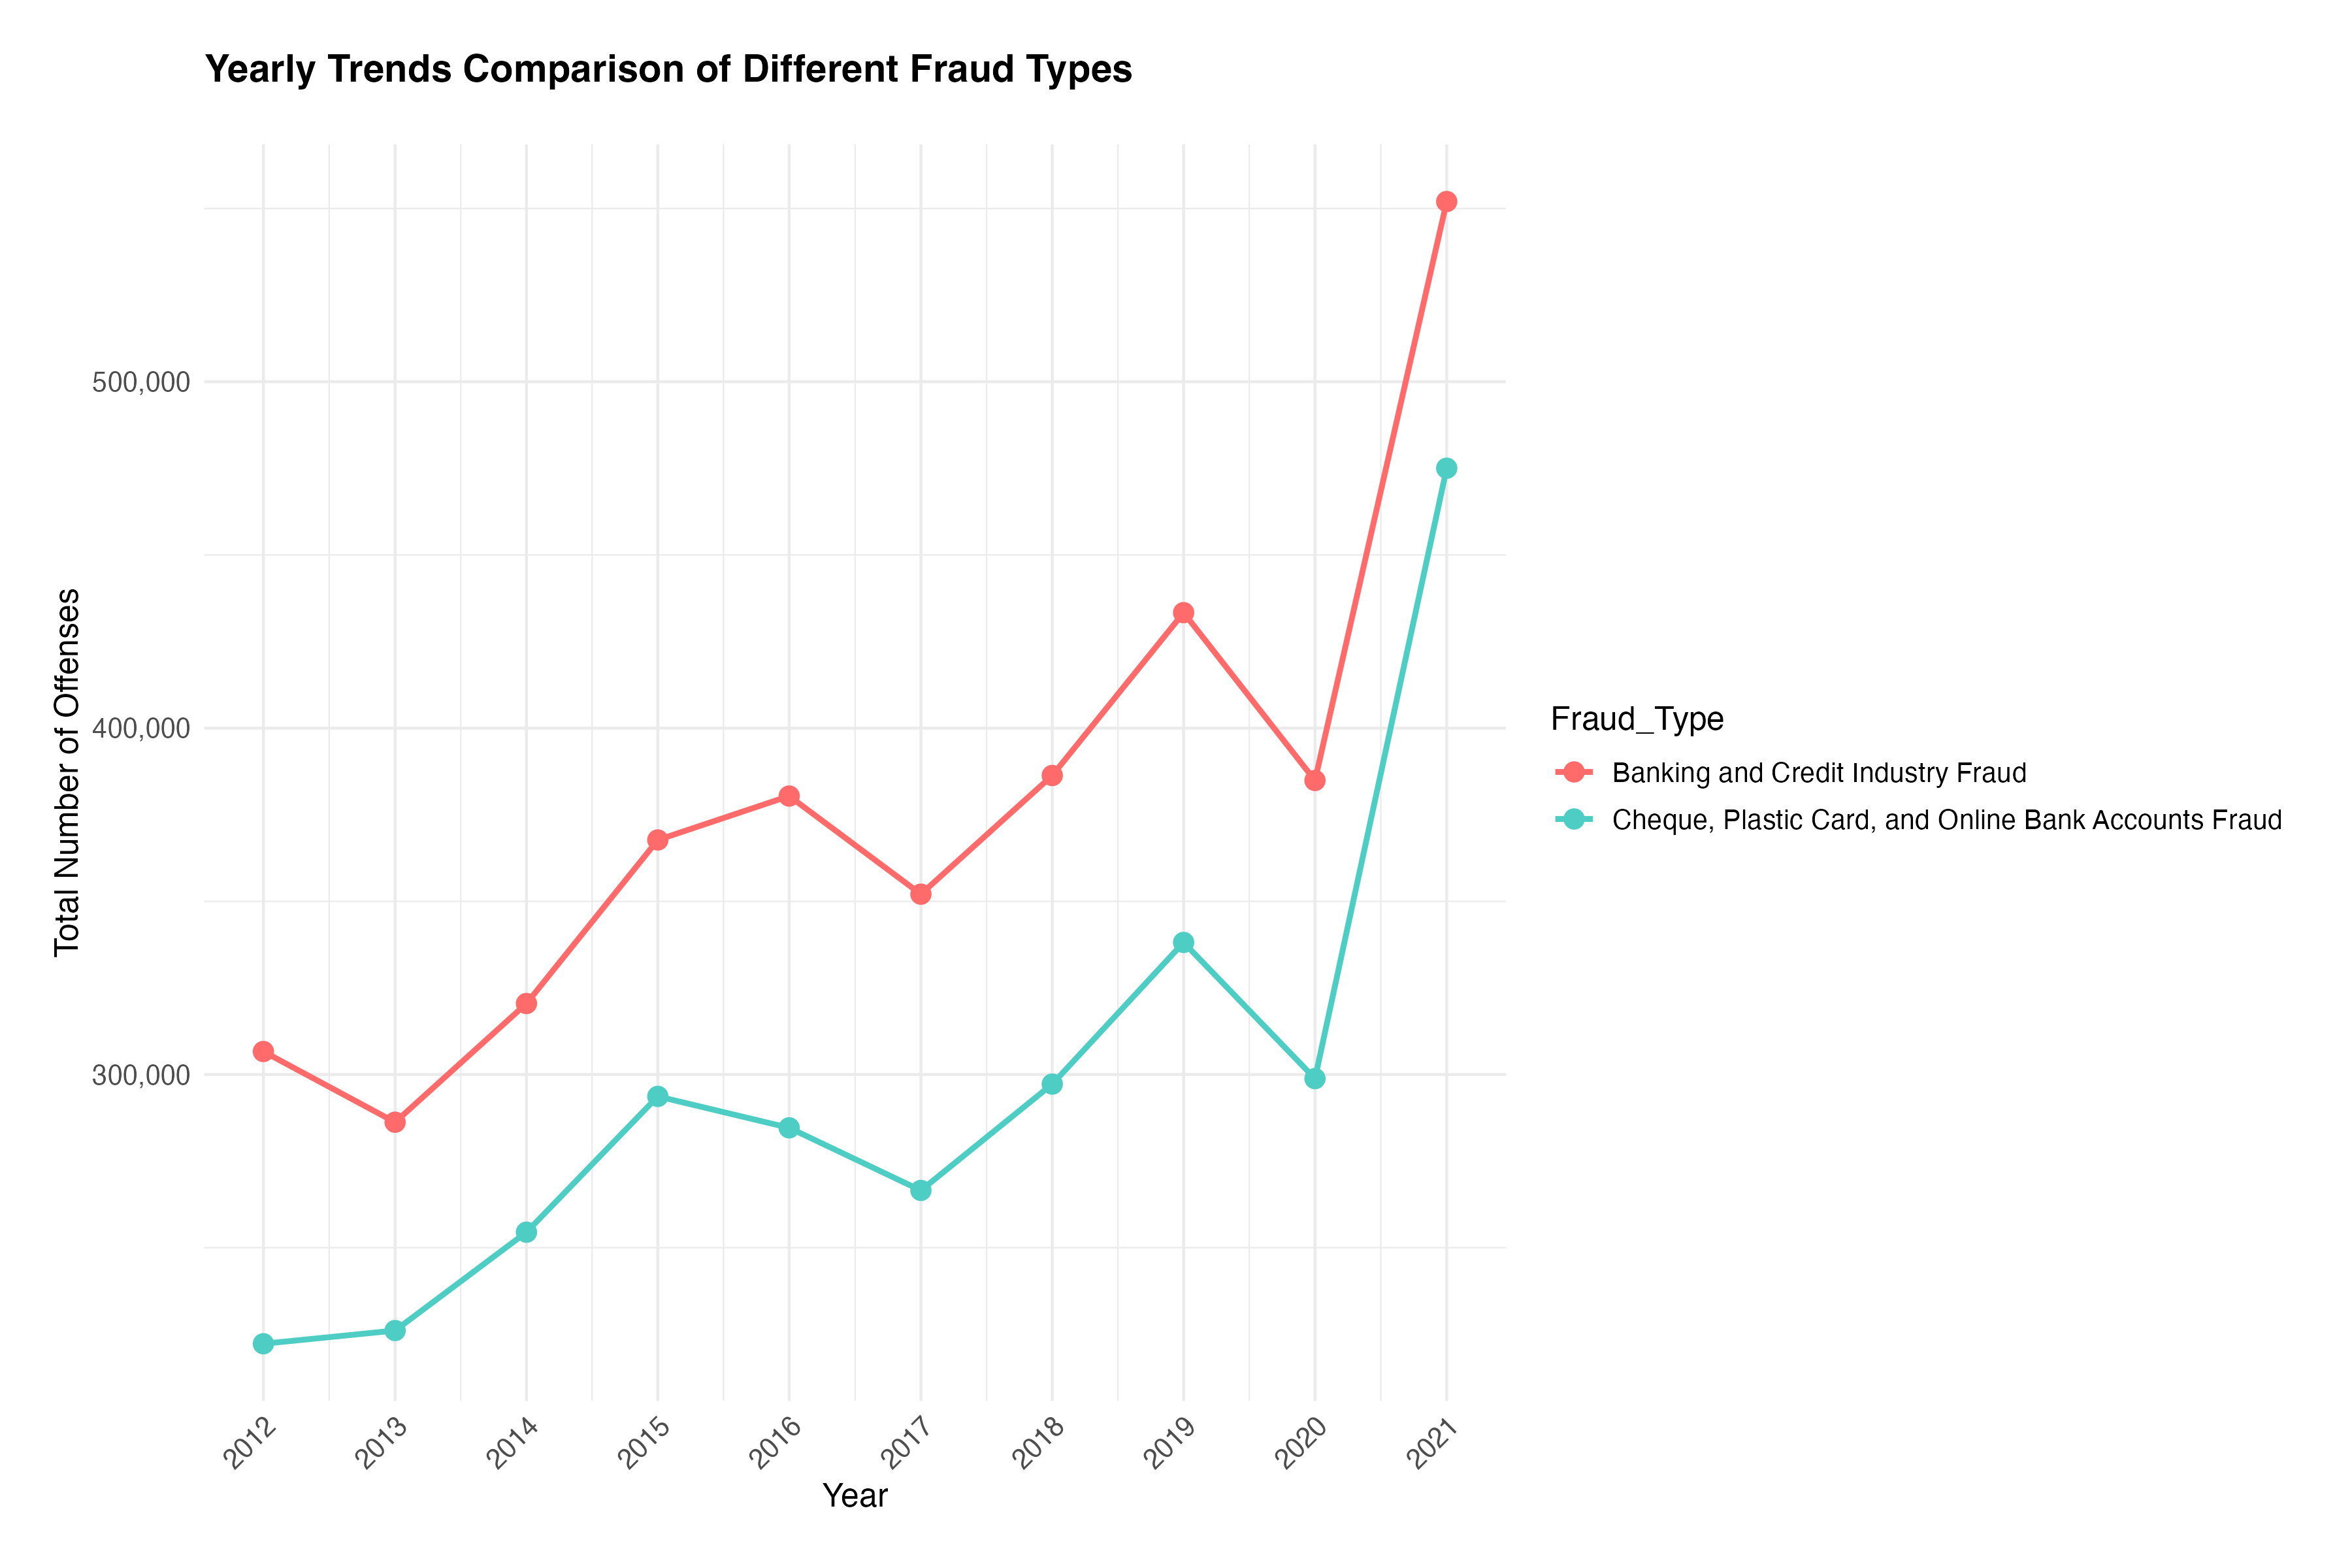
\includegraphics[width=0.7\linewidth]{Images/Plot1.png}
        \caption{Comparison Line Graph}
        \label{fig:comparison_line}
    \end{figure}
    
    The analysis of Banking and Credit Industry Fraud showed a mean of approximately 377,011 offenses across the time period, with a notable increase in recent years. The statistical distribution displayed moderate variability, with values ranging from 286,234 to 552,024 offenses. This trend suggests an overall upward trajectory in this type of fraud.
    
    \item \textbf{Distribution Analysis:} Box plots were generated to examine the statistical distribution of fraud cases. This visualization highlighted that Banking and Credit Industry Fraud showed a higher median value and greater variability in case numbers. The interquartile range for Banking and Credit Industry Fraud spanned from approximately 320,000 to 380,000 cases, while Cheque and Card Fraud showed a tighter distribution.
    
    \begin{lstlisting}[style=RStyle, caption={Distribution Visualization}]
    # Generate distribution visualization
    ggplot(combined_long, aes(x = Type, y = Count, fill = Type)) +
      geom_violin() +
      geom_boxplot(width = 0.1, fill = "white") +
      theme_minimal()
    \end{lstlisting}
    
    \begin{figure}[H]
        \centering
        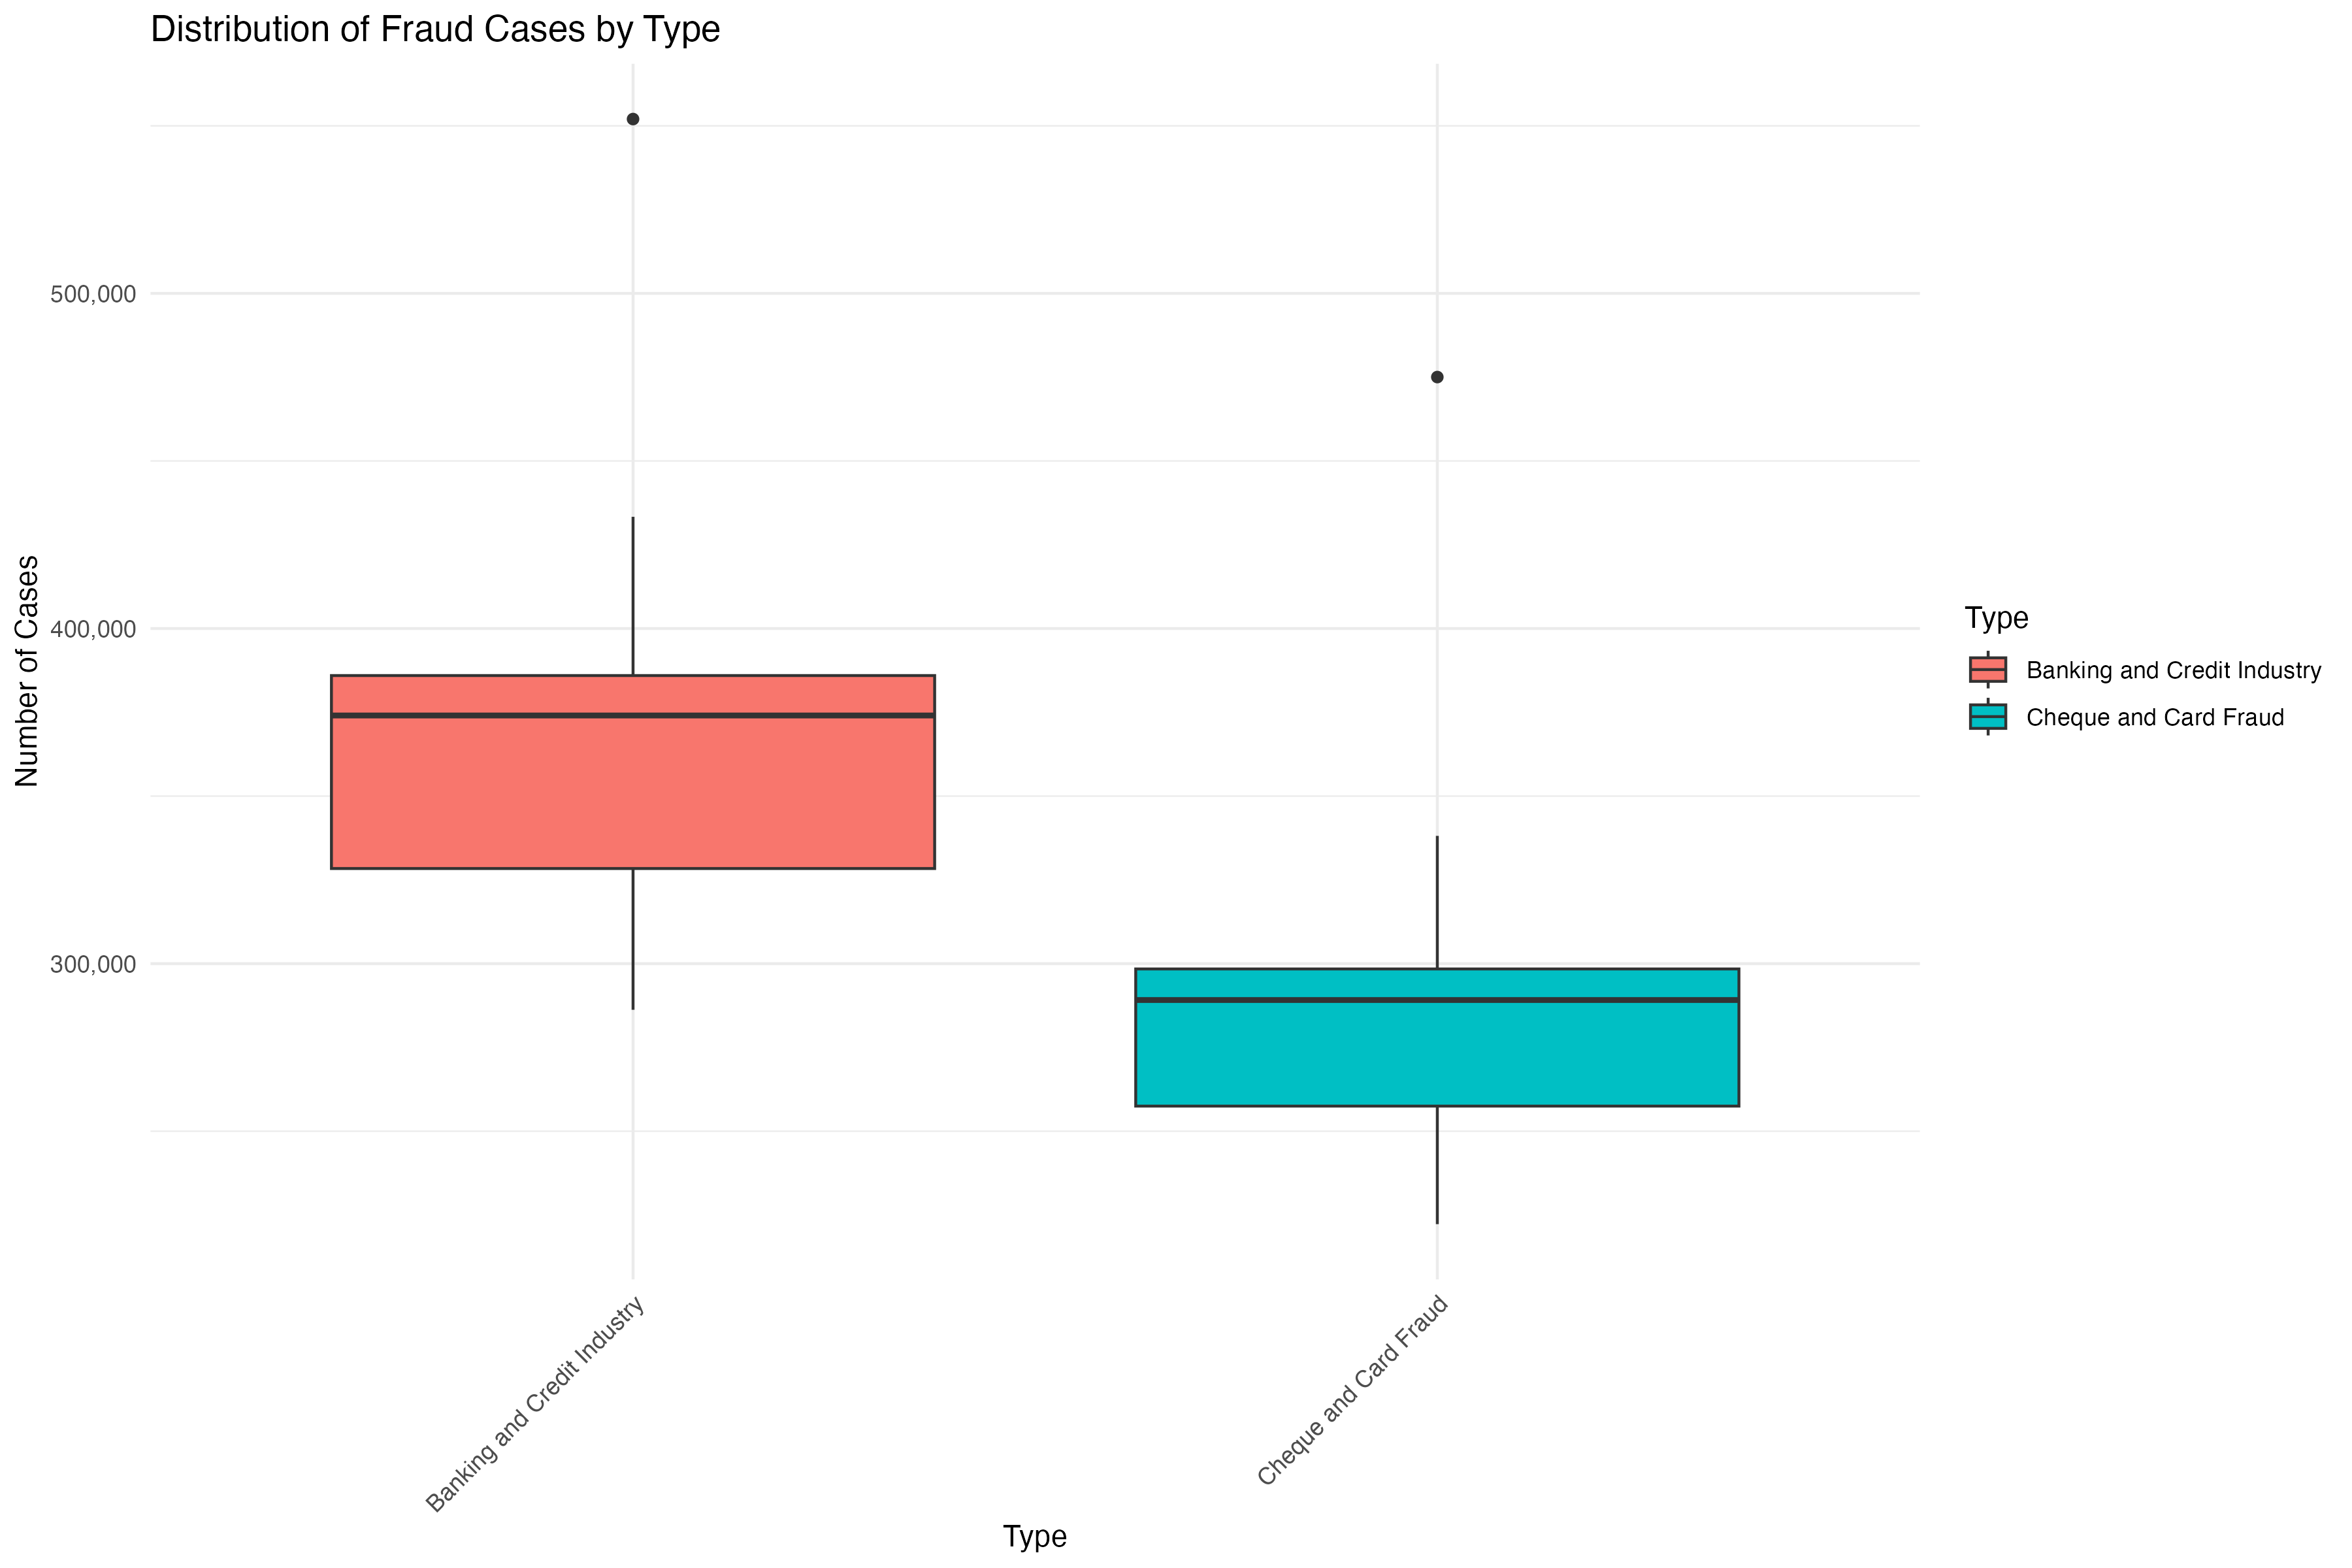
\includegraphics[width=0.7\linewidth]{Images/Plot2.png}
        \caption{Comparison Box Plot}
        \label{fig:comparison_box}
    \end{figure}
    
    For Cheque, Plastic Card, and Online Bank Accounts Fraud, the data revealed a mean of approximately 295,688 offenses, with a median of 293,683. The standard deviation of 65,291 indicates substantial variation in the number of offenses over time. The minimum recorded value was 222,272, while the maximum reached 475,038 offenses, demonstrating significant fluctuation in this category.
    
    \item \textbf{Density Distribution:} A violin plot was implemented to provide deeper insights into the probability density of fraud cases. This revealed interesting patterns in the distribution shapes:
    
    \begin{figure}[H]
        \centering
        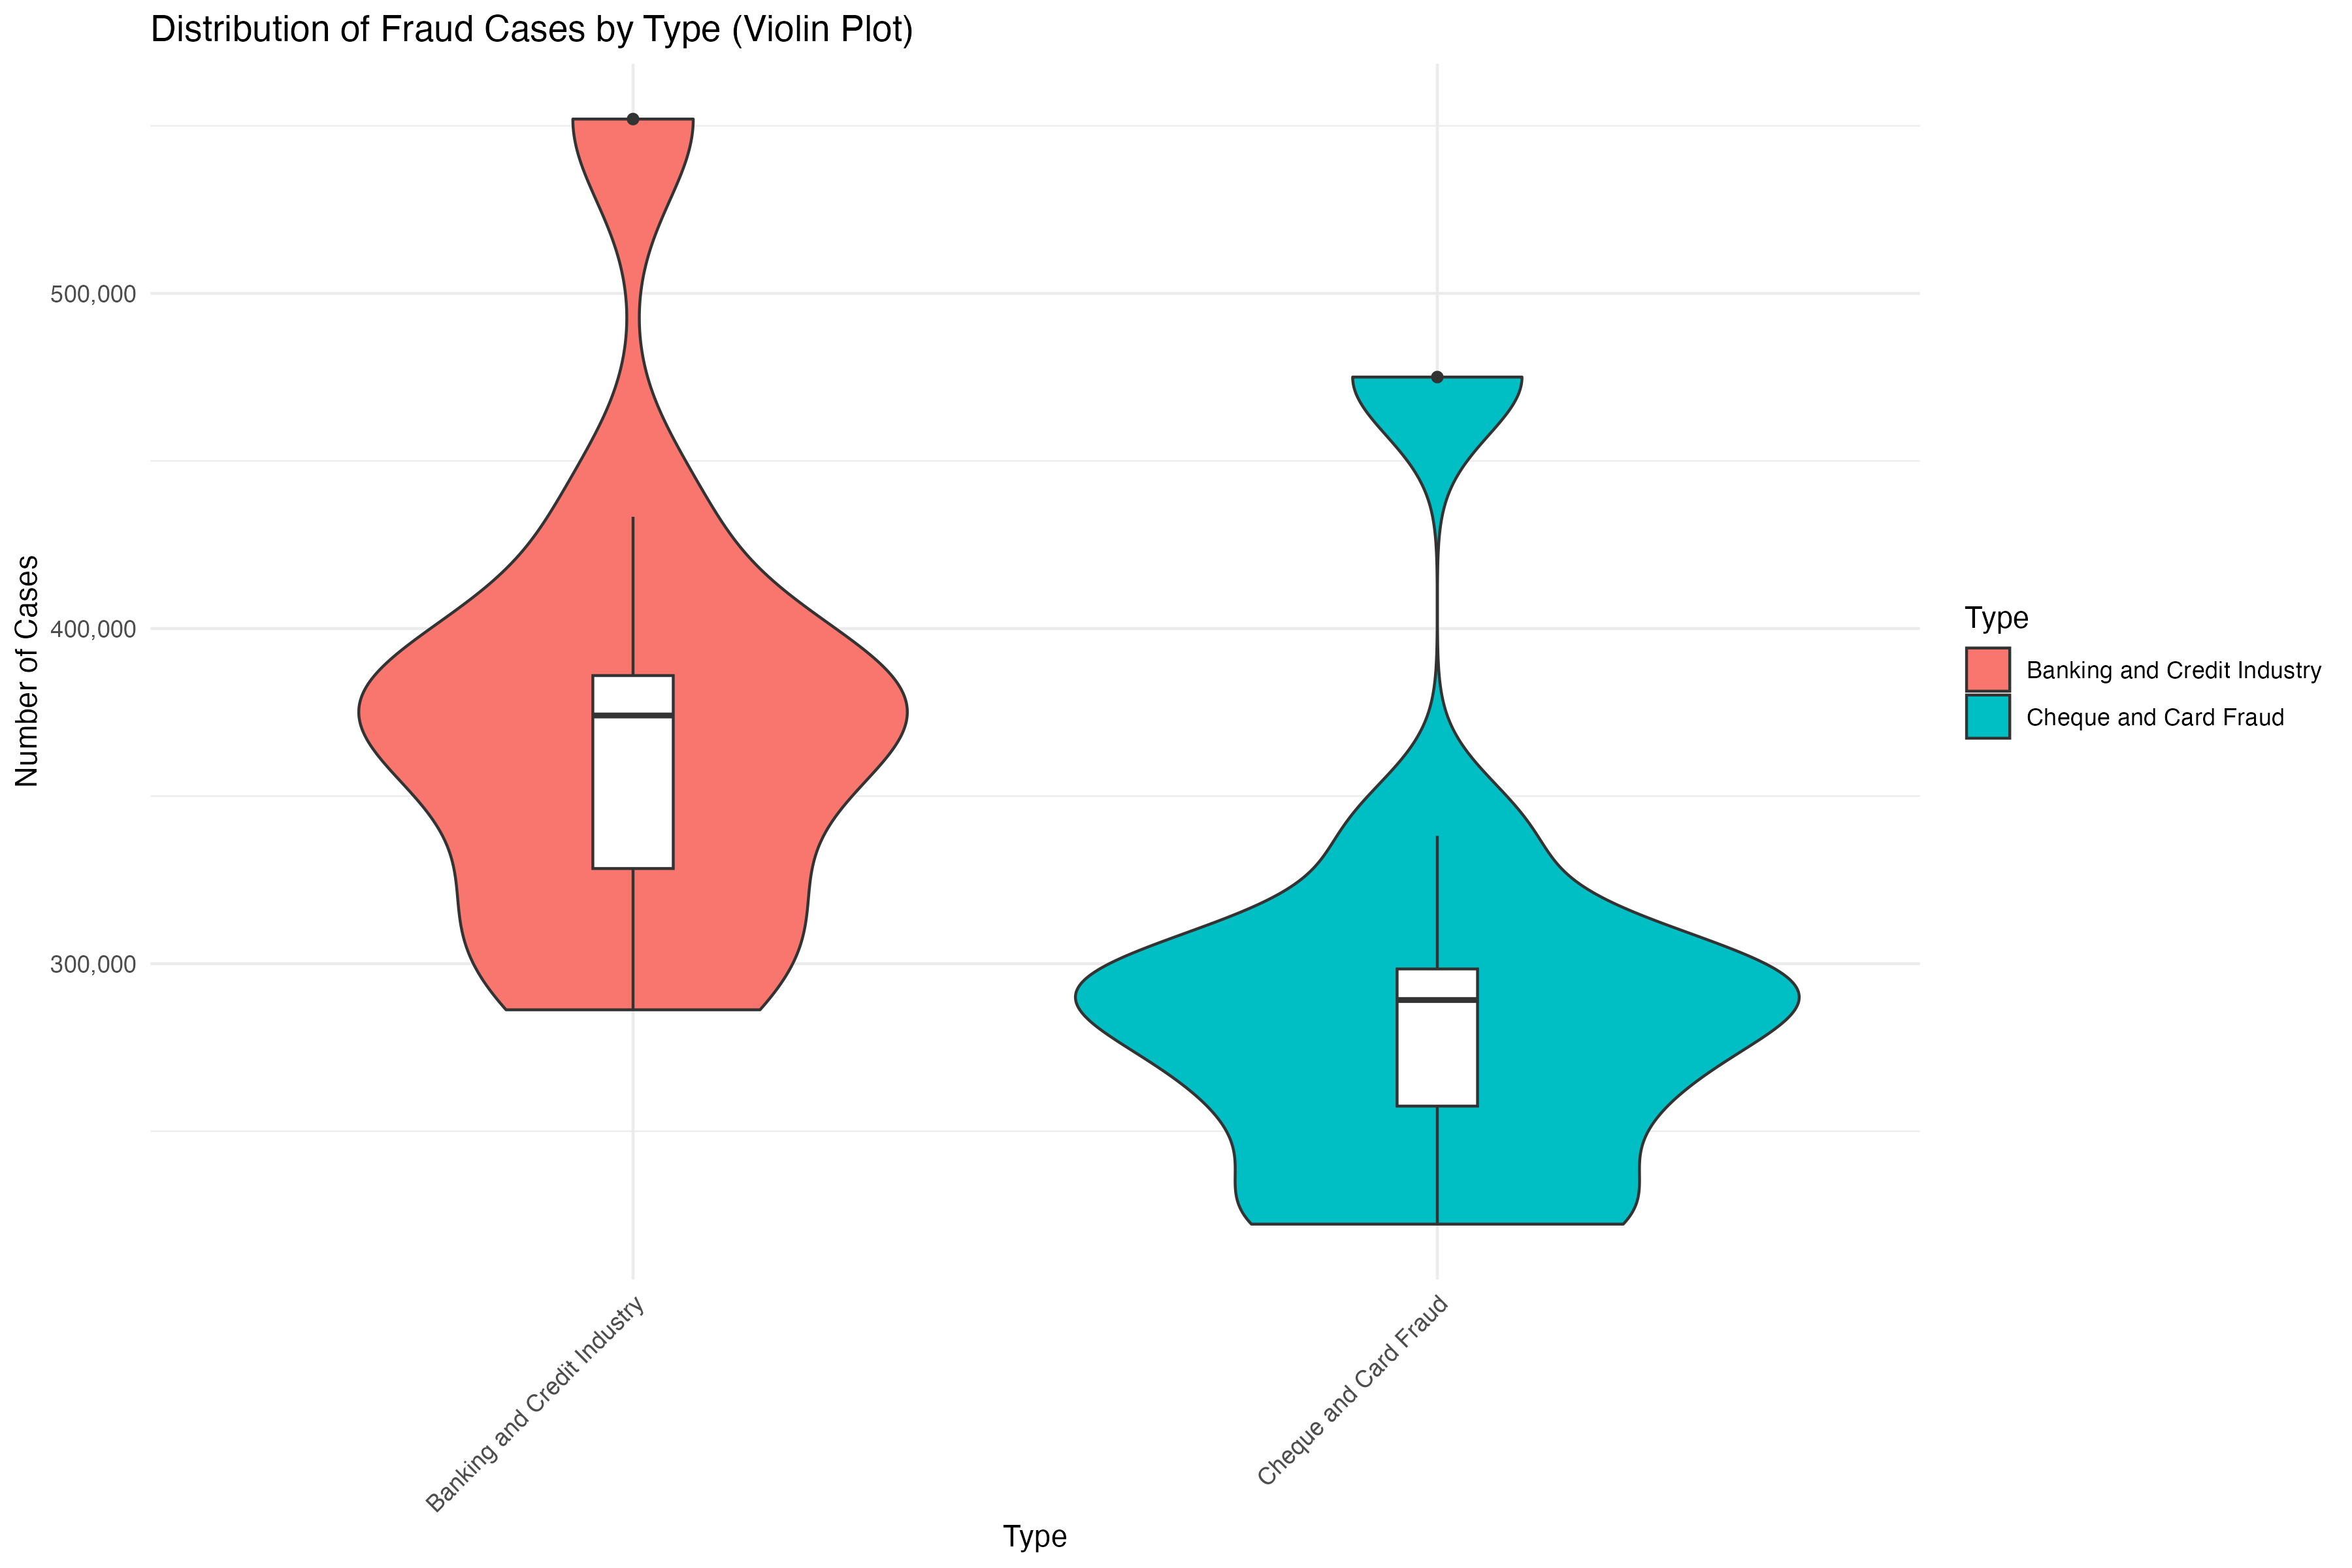
\includegraphics[width=0.7\linewidth]{Images/Plot3.png}
        \caption{Violin Plot with embedded Box Plot}
        \label{fig:violin_plot}
    \end{figure}
    
    \begin{itemize}
        \item Banking and Credit Industry Fraud showed a bimodal distribution, indicating two distinct periods of fraud activity levels
        \item Cheque and Card Fraud displayed a more uniform distribution with a slight positive skew
    \end{itemize}
\end{enumerate}

The violin plot implementation combines both the density distribution visualization and box plot elements to provide a comprehensive view of the fraud data distribution. Here's the essential code for creating this visualization:

\begin{lstlisting}[style=RStyle, caption={Violin Plot Implementation}]
# Generate violin plot with embedded box plot
ggplot(combined_long, aes(x = Type, y = Count, fill = Type)) +
    geom_violin() +
    geom_boxplot(width = 0.1, fill = "white") +
    theme_minimal() +
    ggtitle("Distribution of Fraud Cases by Type") +
    ylab("Number of Cases") +
    theme(axis.text.x = element_text(angle = 45, hjust = 1))
\end{lstlisting}

This code creates a violin plot where the width of each ``violin'' shape represents the probability density of the data at different values. The embedded box plot provides additional statistical information including median, quartiles, and potential outliers. The \texttt{width = 0.1} parameter creates a narrow box plot that doesn't obscure the underlying density distribution, while the white fill helps it stand out against the colored violin plot background.

Moreover, the dispersion and central tendency were visualized using both box plots and violin plots, which effectively illustrated the distribution characteristics of both fraud types. These visualizations highlighted that Banking and Credit Industry Fraud generally maintained higher offense numbers but also showed greater variability compared to Cheque and Card Fraud.

The statistical analysis revealed that Banking and Credit Industry Fraud had a higher mean (377,011) compared to Cheque and Card Fraud (295,688), with both categories showing significant increases in the final year of the dataset.

\subsection{Data Transformation and Visualisation}

The analysis focused on examining fraud patterns across regions and counties in England, considering both absolute numbers of offenses and population-adjusted rates. The investigation revealed notable geographic variations in fraud incidence.

First, the data was prepared by creating appropriately structured dataframes:

\begin{lstlisting}[style=RStyle, caption={Data Preparation and Structure}]
# Create regional and county dataframes
table5_df <- table5_data %>%
 rename(
   Area_Code = `Area Code`,
   Area_Name = `Area Name`,
   Offences = `Number of offences`,
   Rate = `Rate per 1,000 population`
 ) %>%
 filter(!Rate %in% c("[z]", "[u1]")) %>%
 mutate(Rate = as.numeric(Rate))
\end{lstlisting}

The regional analysis revealed distinct patterns in both total offenses and population-adjusted rates. Bar plots were chosen for this visualization as they effectively display comparative magnitudes across categories:

\begin{lstlisting}[style=RStyle, caption={Regional Visualization Code}]
# Create regional visualization
ggplot(regions_df, aes(x = reorder(Area_Name, -Offences), y = Offences)) +
   geom_bar(stat = "identity", fill = "steelblue") +
   theme_minimal() +
   theme(axis.text.x = element_text(angle = 45, hjust = 1)) +
   labs(title = "Total Offences by Region",
        x = "Region",
        y = "Number of Offences")
\end{lstlisting}

\begin{figure}[H]
   \centering
   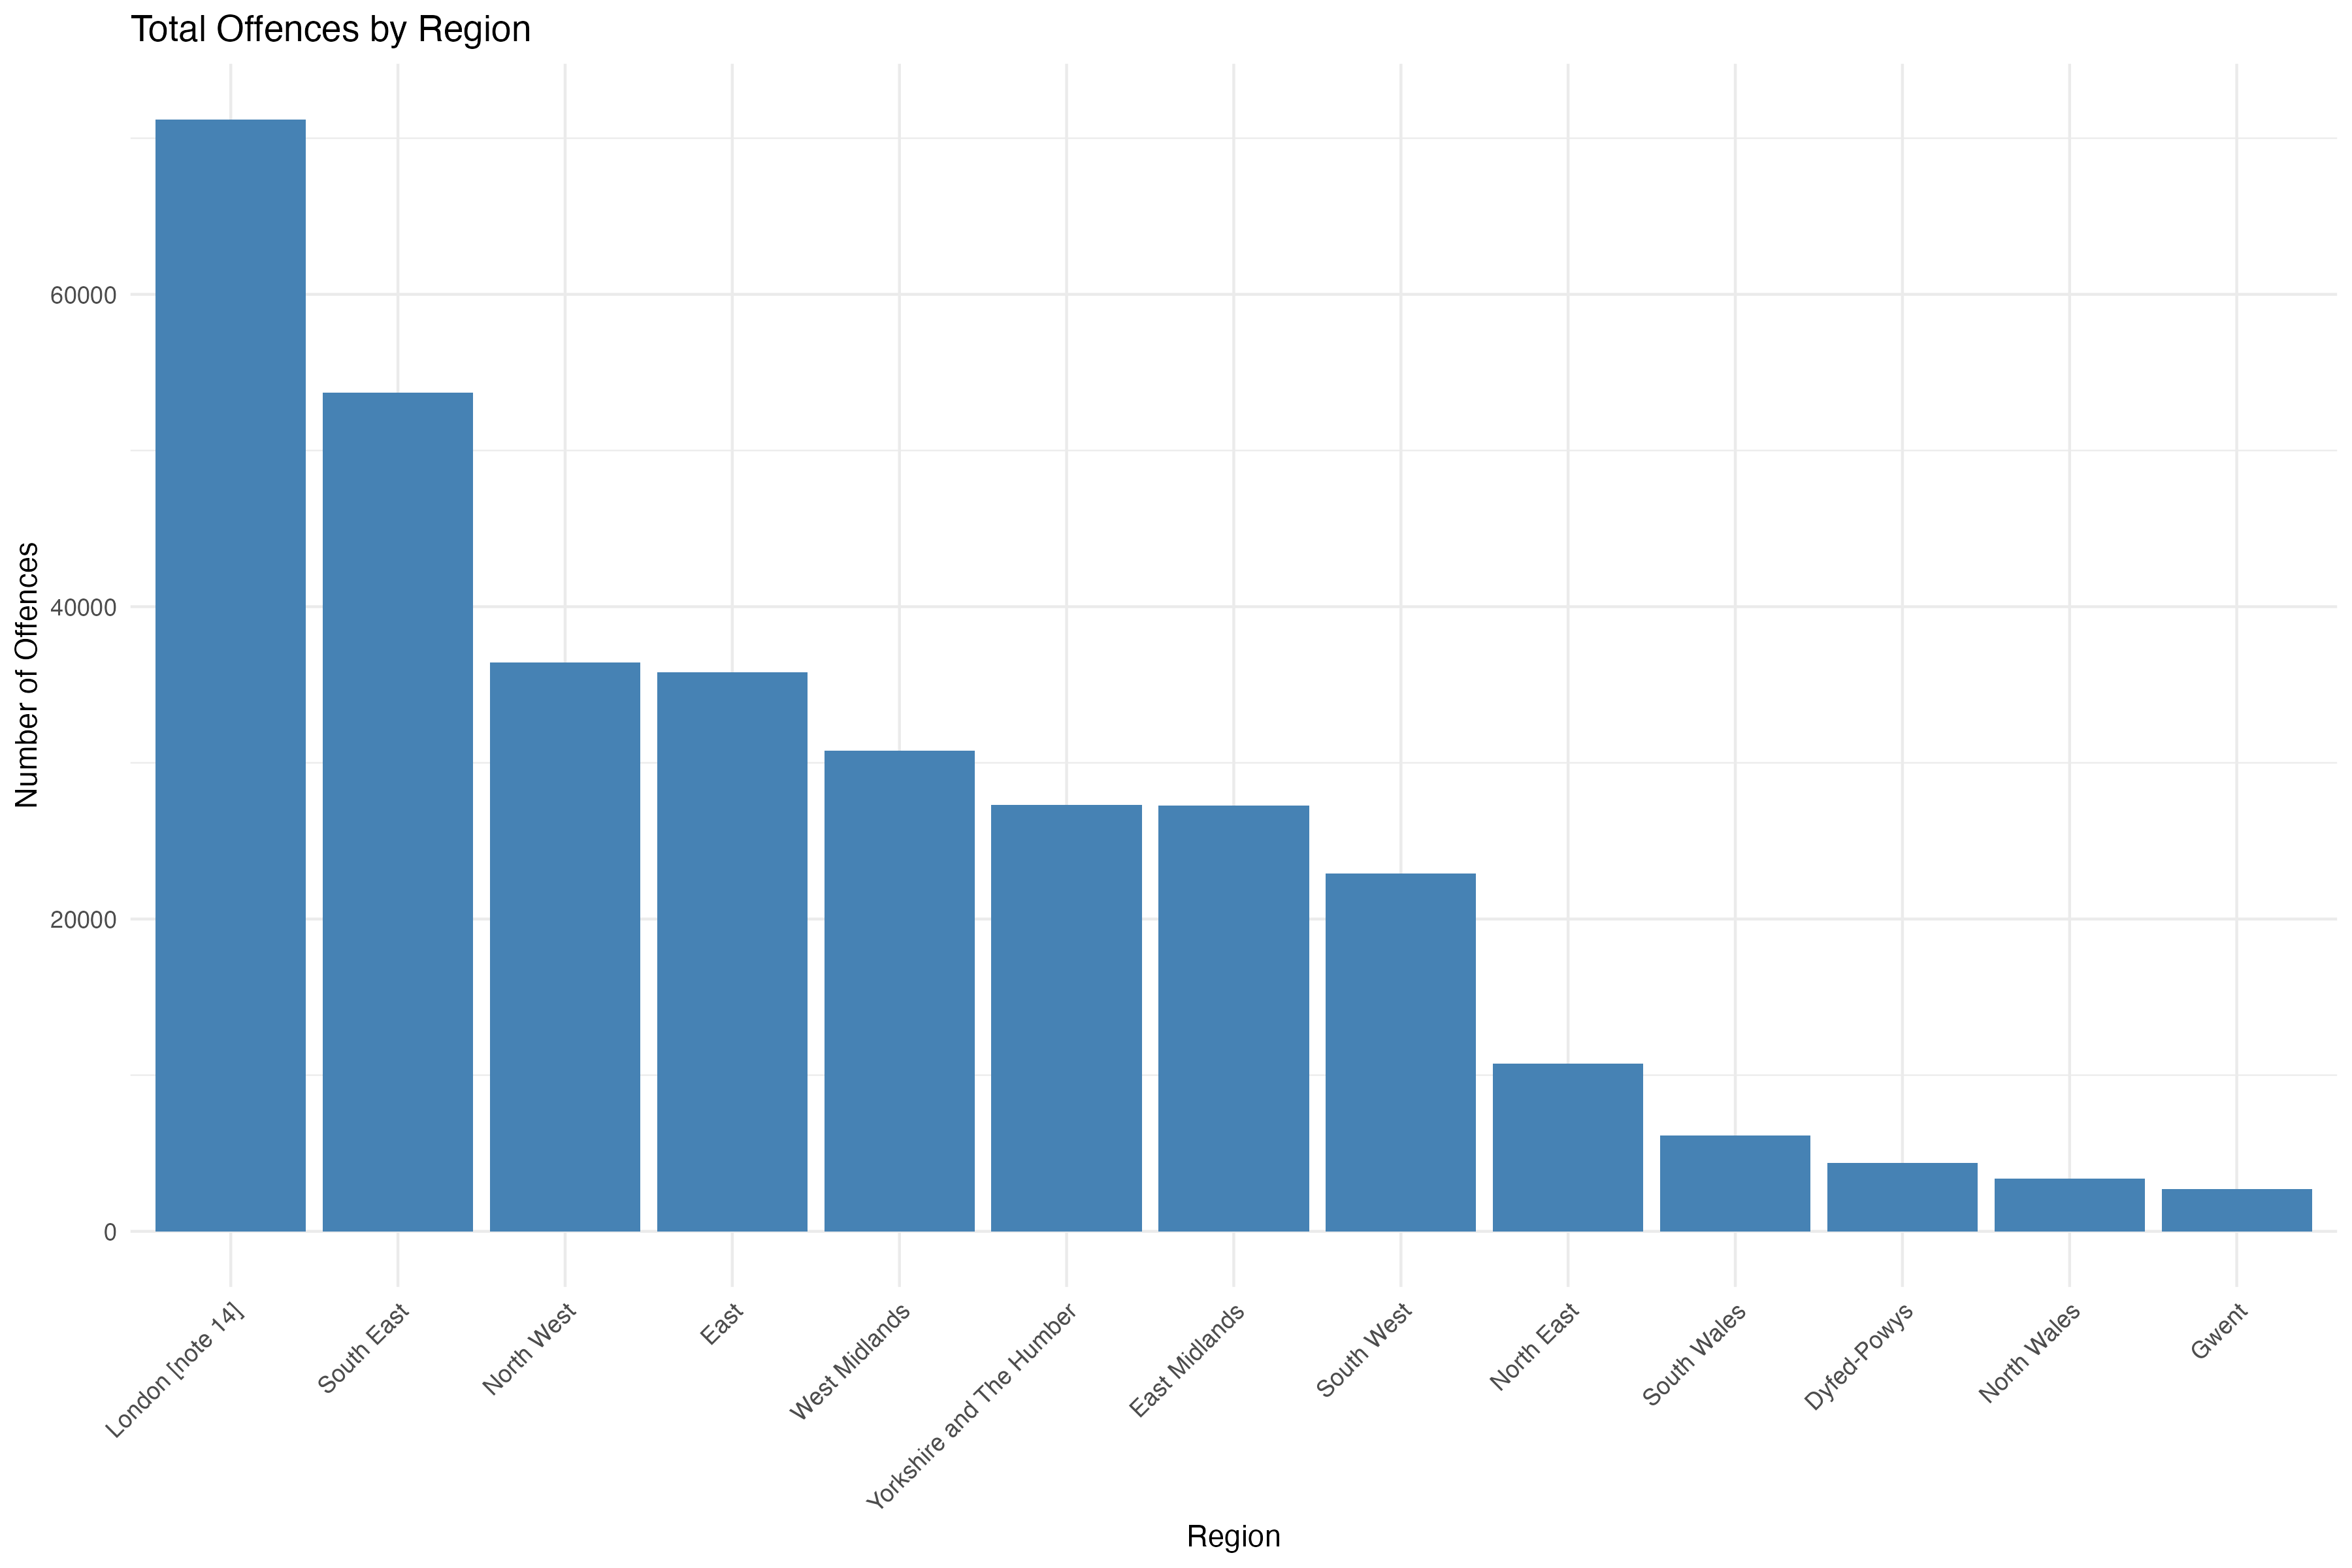
\includegraphics[width=0.7\linewidth]{Images/Plot4.png}
   \caption{Total Offences by Region}
   \label{fig:regional_offences}
\end{figure}

The analysis revealed that London had significantly higher fraud incidence than other regions, with approximately 70,000 offenses, followed by the South East with about 52,000 offenses. However, when examining rates per 1,000 population, Dyfed-Powys showed the highest rate at 8.5, followed by London at 7.9, indicating that raw numbers alone don't tell the complete story of fraud risk.

At the county level, the analysis focused on identifying areas with the lowest fraud incidence. A horizontal bar chart was selected for this visualization to clearly display the ordering of counties:

\begin{lstlisting}[style=RStyle, caption={County-Level Visualization}]
# Create county-level visualization
counties_df %>%
   head(10) %>%
   ggplot(aes(x = reorder(Area_Name, Offences), y = Offences)) +
   geom_bar(stat = "identity", fill = "lightgreen") +
   theme_minimal() +
   coord_flip() +
   labs(title = "10 Counties with Lowest Total Offences",
        x = "County",
        y = "Number of Offences")
\end{lstlisting}

\begin{figure}[H]
   \centering
   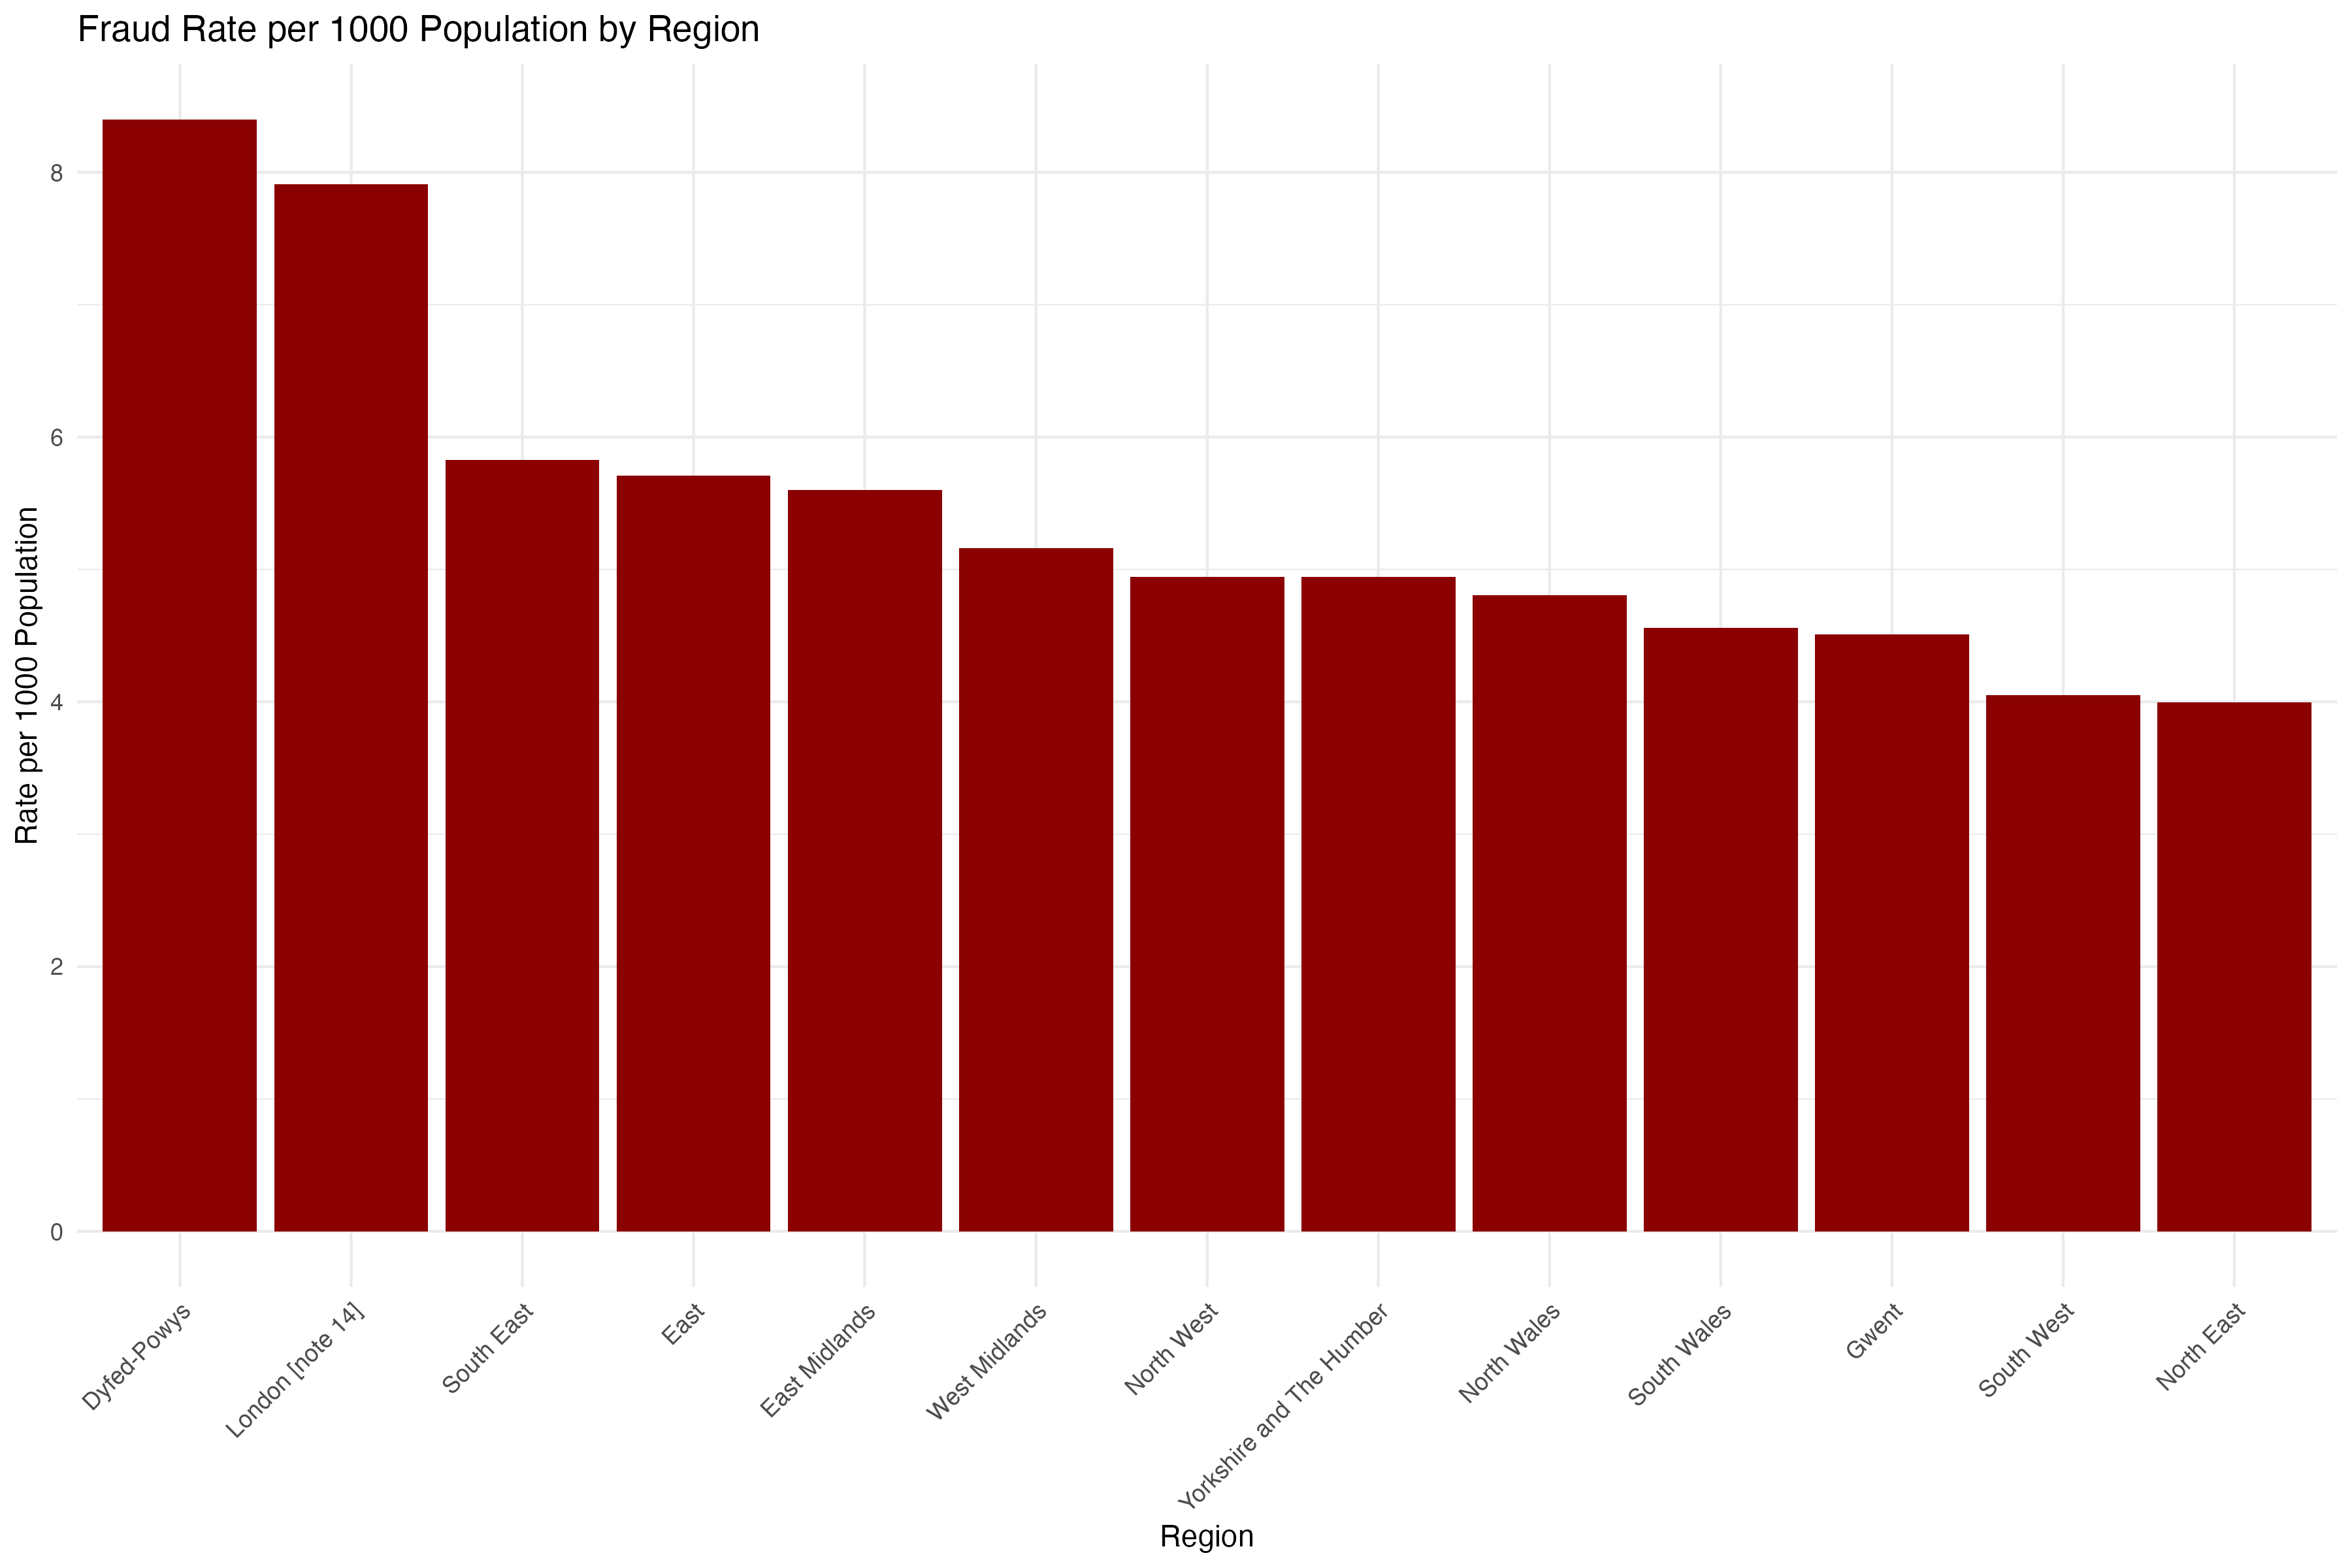
\includegraphics[width=0.7\linewidth]{Images/Plot5.png}
   \caption{Counties with Lowest Total Offences}
   \label{fig:county_offences}
\end{figure}

The visualization revealed that Avon and Somerset had the lowest total count of offenses (2,012), followed by Cumbria (2,134) and Cleveland (2,225). This pattern suggests that rural and less densely populated counties generally experience lower absolute numbers of fraud offenses, though this doesn't necessarily indicate lower risk when adjusted for population size.

\begin{lstlisting}[style=RStyle, caption={Enhanced County Visualization}]
# Create visualization for lowest offense counties
counties_df %>%
   head(10) %>%
   ggplot(aes(x = reorder(Area_Name, Offences), y = Offences)) +
   geom_bar(stat = "identity", fill = "lightgreen") +
   theme_minimal() +
   theme(
       panel.grid.minor = element_blank(),
       axis.text.x = element_text(angle = 45, hjust = 1),
       plot.title = element_text(hjust = 0.5, margin = margin(b = 20))
   ) +
   labs(
       title = "10 Counties with Lowest Total Offences",
       x = "County",
       y = "Number of Offences"
   )
\end{lstlisting}

\begin{figure}[H]
   \centering
   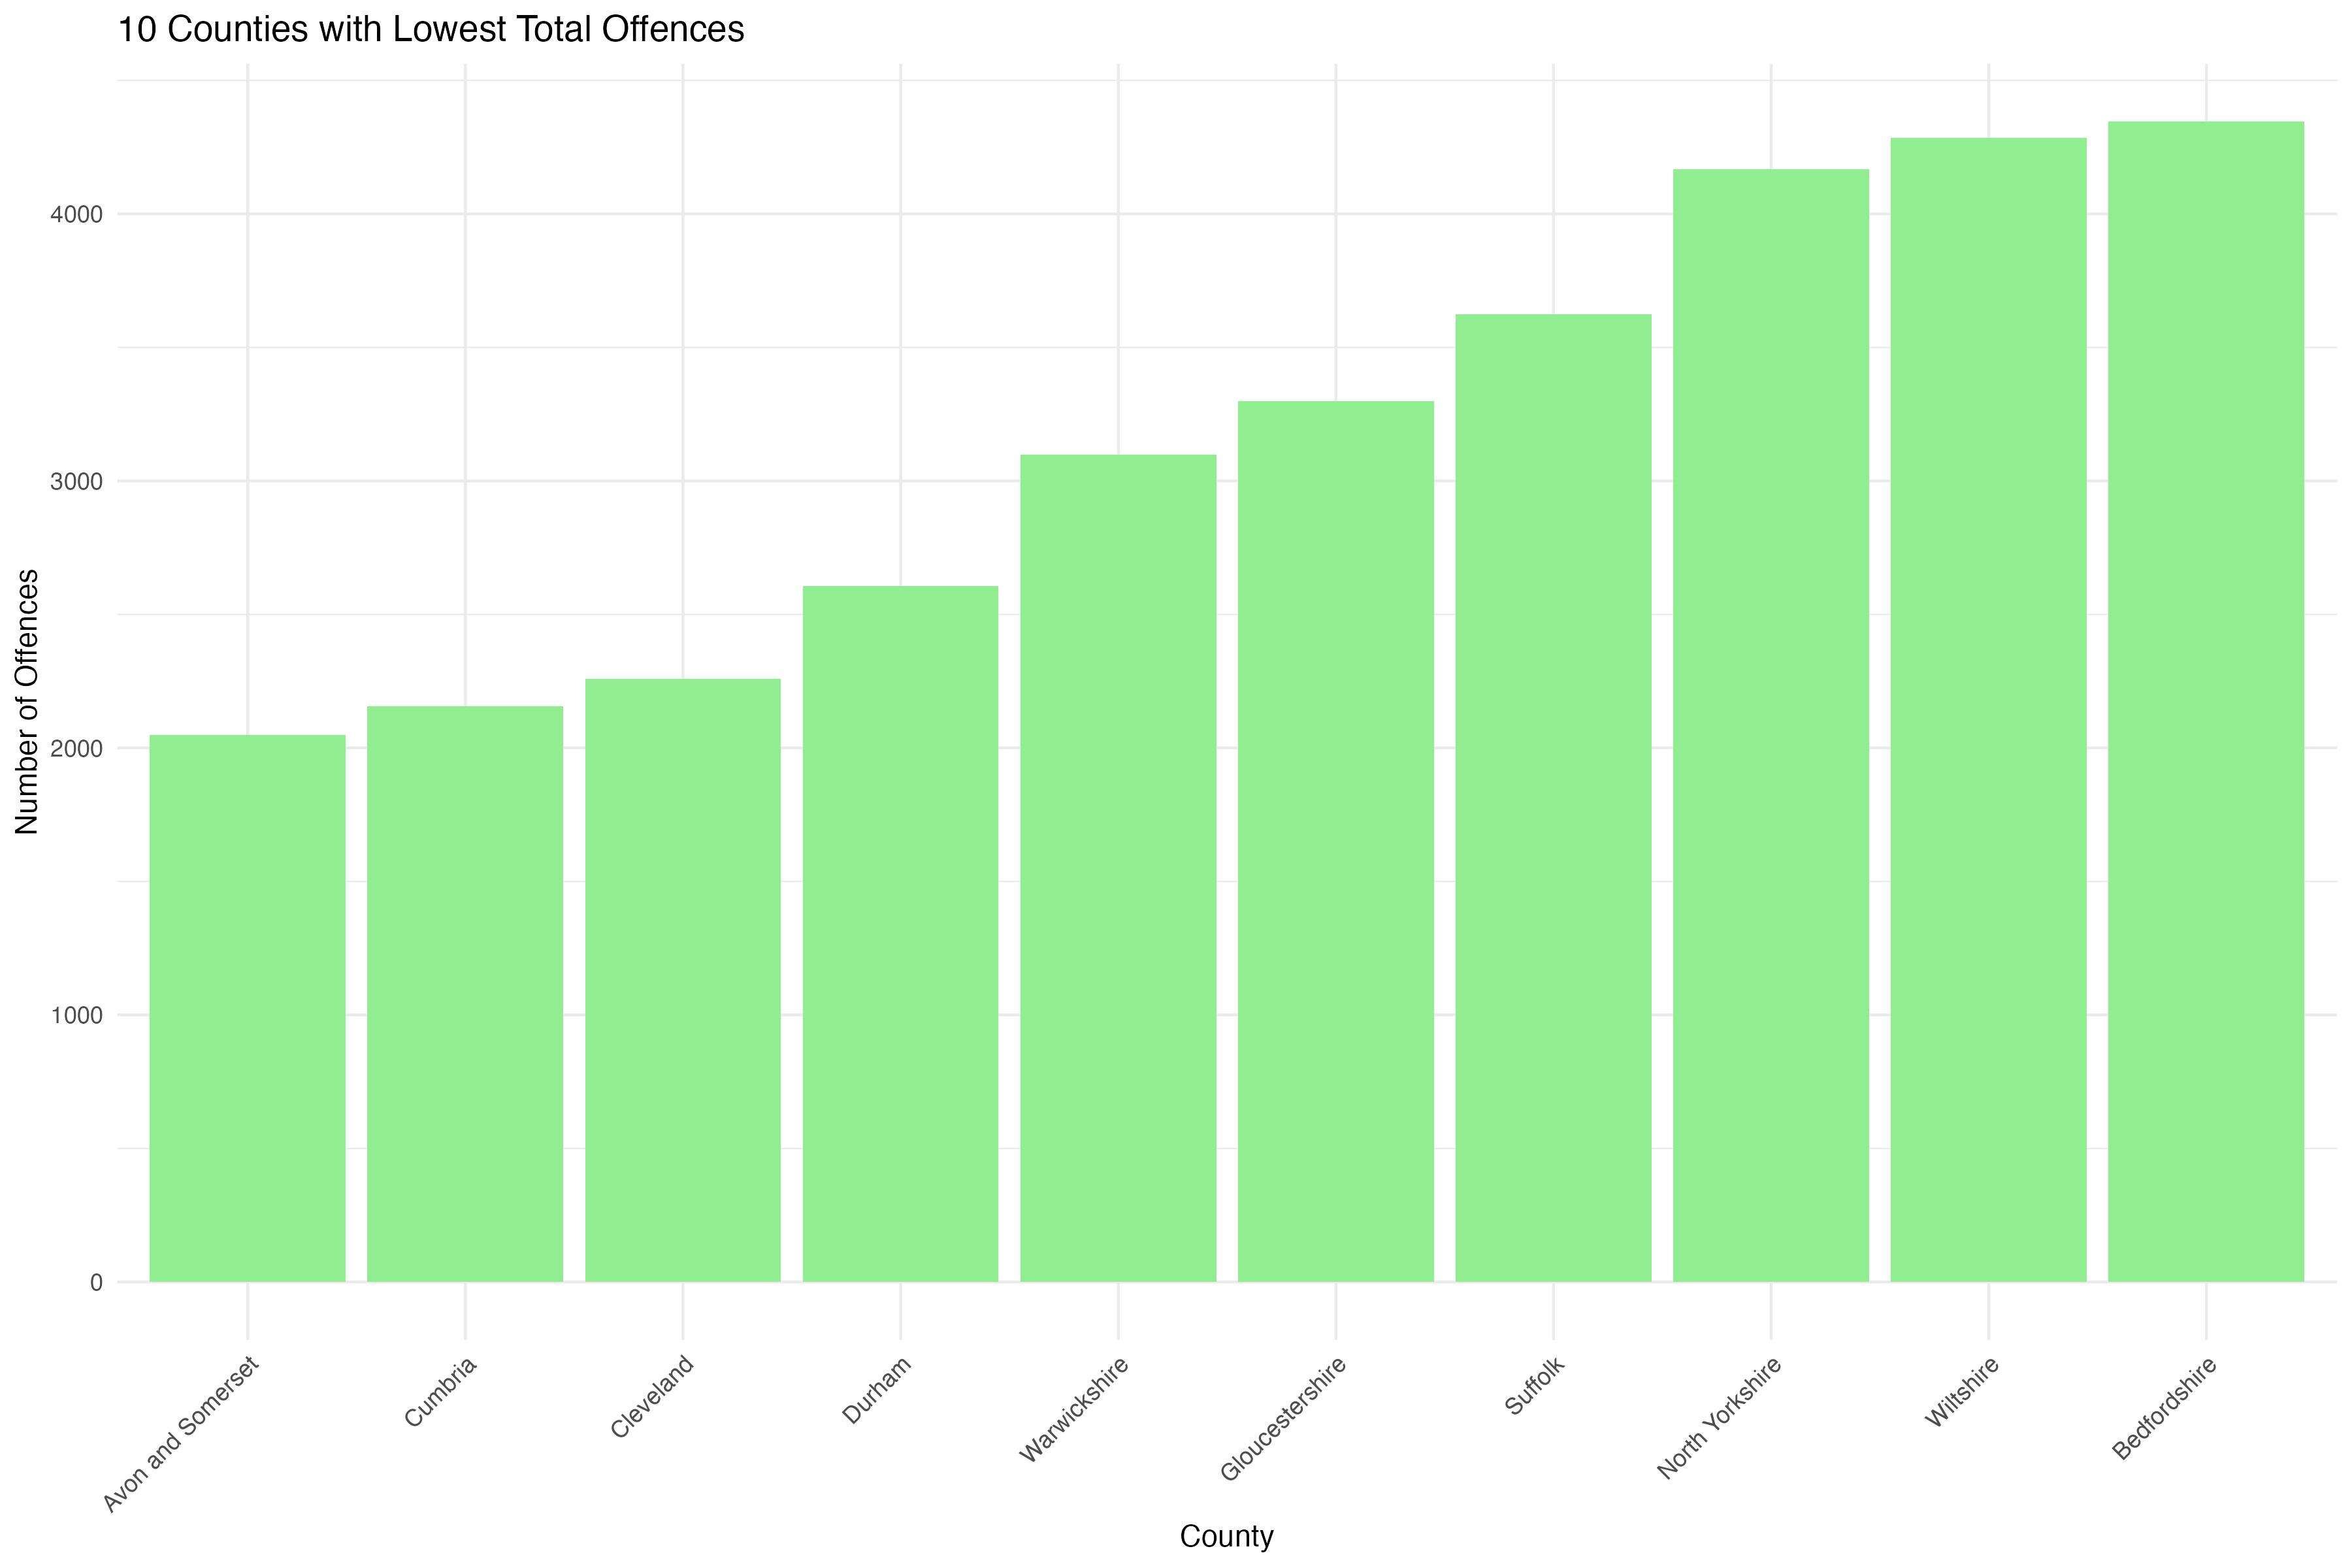
\includegraphics[width=0.7\linewidth]{Images/Plot6.png}
   \caption{Enhanced Visualization of Counties with Lowest Offences}
   \label{fig:enhanced_county_offences}
\end{figure}

The choice of bar plots for both regional and county-level analysis was driven by their effectiveness in comparing quantities across categories. The horizontal orientation for county-level data improved readability given the larger number of categories, while color coding (\texttt{steelblue} for regions, \texttt{lightgreen} for counties) helped distinguish between the two geographic levels of analysis.

% \printbibliography
\end{document}
